\section{DA Wandler}\hartl{455}
\subsection{Lernziele}
\begin{itemize}
  \item Strom-Spannungs-DAC
  \item DAC Grundprinzipien
  \begin{itemize}
    \item Parallelverfahren  
    \item Wägeverfahren
    \item Zählverfahren
   \end{itemize}
  \item Kombinierte Wandler
\end{itemize}

\subsection{Parallelverfahren (Voltage Scaling)}
\begin{longtable}{|l|l|l|}
\hline
\begin{minipage}{4cm}
\textbf{Strom-DAC} \hartl{456}
\end{minipage}
&
\begin{minipage}{6cm}
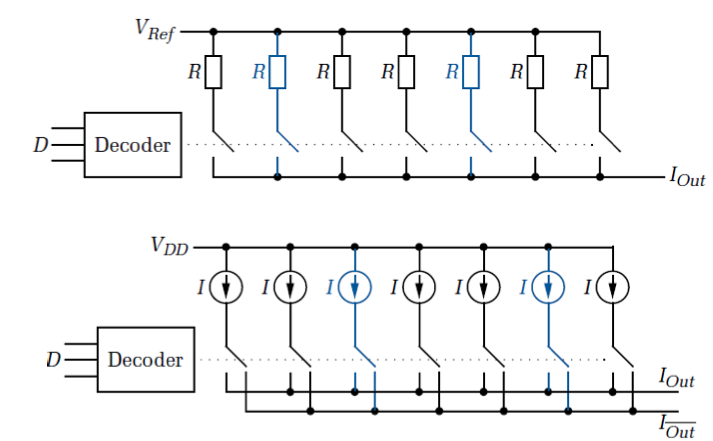
\includegraphics[width=6cm, height = 4.5cm]{pictures/Strom-DAC}
\end{minipage}

&
\begin{minipage}{8cm}
\begin{gather}
K=2^N-1\\
I=\frac{V_{Ref}}{R}\\
I_{Out}=D*I=D*\frac{V_{Ref}}{R}\\
I_{Out}=D*I\\
I_{\bar{Out}}=(K-D)*I\\
V_{Out}=RI_{Out}-RI_{\bar{Out}}\notag\\=(D-K)*RI
\end{gather}
\begin{tabular}{ll}
K:&Anzahl Stromquellen\\
D:&Eingangswert\\&(Anzahl Schalter die \\&aktiv sind..)
\end{tabular}
\end{minipage}

\\
\hline
\begin{minipage}{4cm}
\textbf{String DAC} \hartl{459}
\end{minipage}
&
\begin{minipage}{6cm}
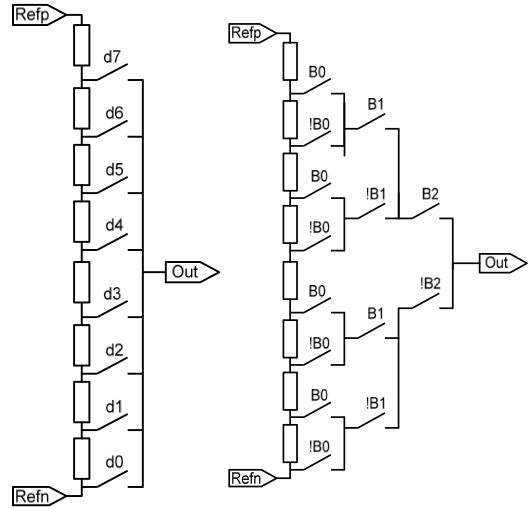
\includegraphics[width=6cm,height=5cm]{pictures/string_DAC}
\end{minipage}&
\begin{minipage}{8cm}
\textbf{Vorteil}
\begin{itemize}
  \item garantierte Stetigkeit
\end{itemize}
\textbf{Nachteil}
\begin{itemize}
  \item benötigt $2^n$ Widerstände und $2^n$ Schalter, n-to-$2^n$ Decoder(linke
  Variante)
  \item $V_{out}(D) = \frac{D}{2^n}(V_{Ref+} -V_{Ref-}) + V_{Ref-}$
\end{itemize}
\end{minipage}
\\
\hline
\begin{minipage}{4cm}
\textbf{Segmented String DAC} \hartl{459}
\end{minipage}
&
\begin{minipage}{6cm}
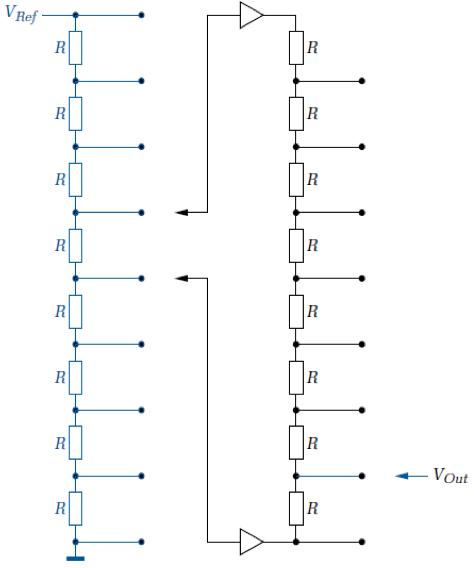
\includegraphics[width=6cm,height=5cm]{pictures/segmented_string_DAC}
\end{minipage}&
\begin{minipage}{8cm}
\textbf{Vorteil}
\begin{itemize}
  \item viel weniger Elemente
\end{itemize}
\textbf{Nachteil}
\begin{itemize}
  \item benötigt Buffer (offset-frei)
\end{itemize}
\end{minipage}
\\
\hline
\begin{minipage}{4cm}
\textbf{Digitales Potentiometer} \hartl{460}
\end{minipage}
&
\begin{minipage}{6cm}
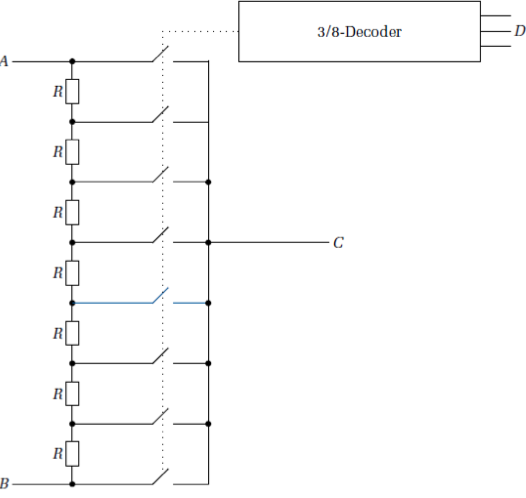
\includegraphics[width=6cm,height=5cm]{pictures/digitales_potentiometer}
\end{minipage}&
\begin{minipage}{8cm}
\textbf{Vorteil}
\begin{itemize}
  \item automatisierter Elektronik-Test möglich
\end{itemize}
\end{minipage}
\\
\hline
\end{longtable}

\subsection{Wägeverfahren} \hartl{461}
\begin{longtable}{|l|l|l|}
\hline
\begin{minipage}{4cm}
\textbf{Spannungs-summierung} \hartl{461}
\end{minipage}
&
\begin{minipage}{6cm}
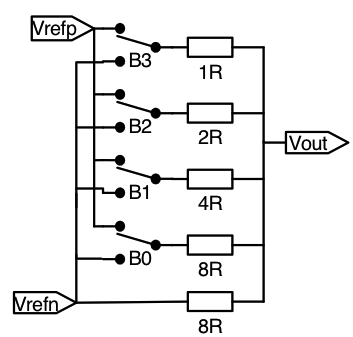
\includegraphics[width=6cm, height = 4.5cm]{pictures/spannungssummierung}
\end{minipage}
&
\begin{minipage}{8cm}
\begin{gather}
V_{Out}=\notag\\=\frac{B0*2^0*G0+B1*2^1*G0}{2^4*G0}*\notag\\
* \frac{B2*2^2*G0+B3*2^3*G0}{2^4*G0}*\notag\\
*(V_{rep}-V_{refn})+V_{refn}
\end{gather}
\textbf{Vorteil}
\begin{itemize}
  \item N Widerstände, N Schalter
\end{itemize}
\textbf{Nachteil}
\begin{itemize}
  \item nicht garantiert stetig
  \item grosse Wertebereiche der Widerstände notwendig
\end{itemize}
\begin{itemize}
  \item rechnen mit Leitwerten
  \item Substitution: $G0=\frac{1}{8R}$
\end{itemize}
\end{minipage}
\\

\hline
\begin{minipage}{4cm}
\textbf{Stromsummierung} \hartl{462}
\end{minipage}
&
\begin{minipage}{6cm}
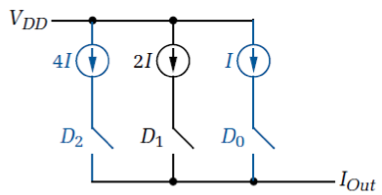
\includegraphics[width=6cm, height = 3.5cm]{pictures/stromsummierung}
\end{minipage}
&
\begin{minipage}{8cm}
\begin{equation}
V_{Out}=(4+1)*I
\end{equation}
\end{minipage}
\\

\hline
\begin{minipage}{4cm}
\textbf{Praktisch}
\end{minipage}
&
\begin{minipage}{6cm}
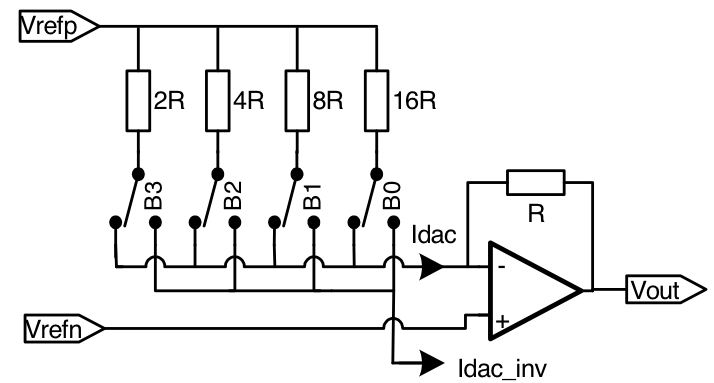
\includegraphics[width=6cm, height = 3.5cm]{pictures/praktisch}
\end{minipage}
&
\begin{minipage}{8cm}
\begin{equation}
Idac_{max}=\frac{V_{refp}-V_{refn}}{R}*\frac{2^n-1}{2^n}
\end{equation}
\end{minipage}
\\
\hline

\hline
\begin{minipage}{4cm}
\textbf{R-2R-Netzwerk} \hartl{462}
\end{minipage}
&
\begin{minipage}{6cm}
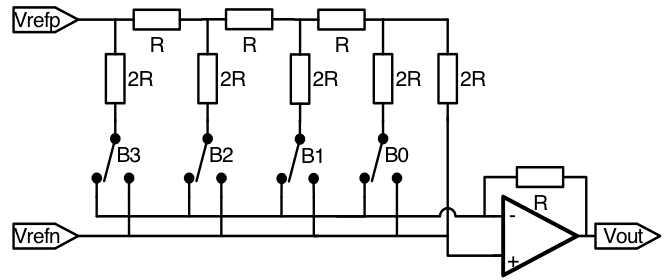
\includegraphics[width=6cm, height = 3.5cm]{pictures/r2rnetzwerk}
\end{minipage}
&
\begin{minipage}{8cm}


\end{minipage}
\\
\hline

\begin{minipage}{4cm}
\textbf{kapazitiver DAC}
\end{minipage}
&
\begin{minipage}{6cm}
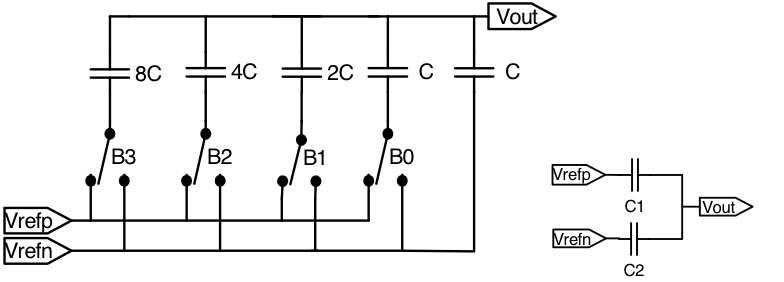
\includegraphics[width=6cm, height = 3.5cm]{pictures/kapazitiverDAC}
\end{minipage}
&
\begin{minipage}{8cm}
\begin{gather}
C1=B3\cdot 8C+B2\cdot 4C+\notag\\+B1\cdot 2C+B0\cdot C\\
C2=!B3\cdot 8C+!B2\cdot 4C+\notag\\+!B1\cdot 2C+!B0\cdot C+C\\
V_{Out}=\frac{C1}{C1+C2}\cdot (V_{refp}-V_{refn})\\
\text{mit } C1+C2=2^n\cdot C
\end{gather}

\end{minipage}
\\
\hline
\end{longtable}
\newpage

\subsection{Zählverfahren(PWM)} \hartl{466}\\
\begin{longtable}{|l|l|l|}
\hline
\begin{minipage}{4cm}
\textbf{Grundprinzip} \hartl{466}
\end{minipage}
&
\begin{minipage}{6cm}
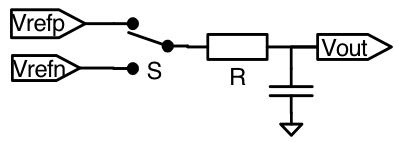
\includegraphics[width=6cm, height = 3cm]{pictures/pwm_DAC}
\end{minipage}
&

\begin{minipage}{8cm}
\begin{gather}
V_{Out}=\frac{D}{2^n}*(V_{refp}-V_{refn})+V_{refn}
\end{gather}
\\
\textbf{Vorteil}
\begin{itemize}
  \item sehr einfache Schaltung
  \item ermöglicht hohe Auflösung
  \item Funktioniert ohne analoge Schaltungen onchip (z.B mit
  FPGA,Microcontroller)
\end{itemize}
\textbf{Nachteil}
\begin{itemize}
  \item sehr langsam
  \item benötigt grosse Zeitkonstanten (Kapazitäg offchip)
\end{itemize}
\end{minipage}
\\
\hline
\begin{minipage}{4cm}
\textbf{PWM-Ansteuerung} \hartl{466}
\end{minipage}
&
\begin{minipage}{6cm}
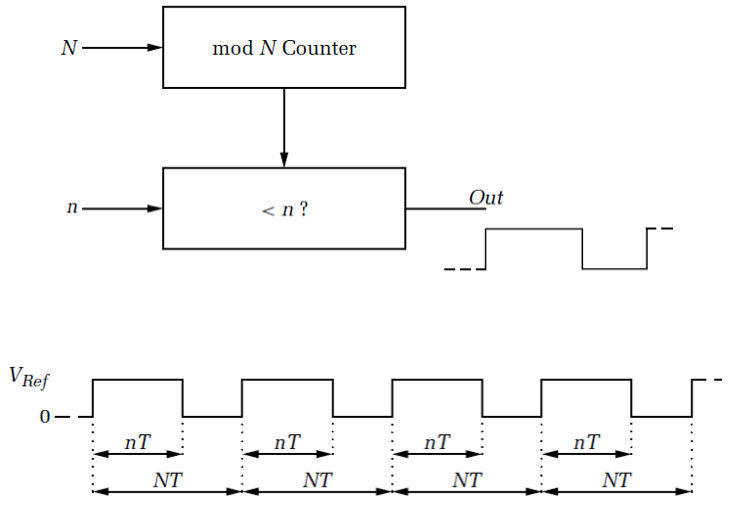
\includegraphics[width=6cm, height = 4cm]{pictures/pwm_Ansteuerung}
\end{minipage}
&

\begin{minipage}{8cm}
\begin{equation}
\bar{V_{Out}}=\frac{n}{N}V_{Ref}
\end{equation}
\begin{tabular}{ll}
N:&Takte\\
n:&digitale Eingangsgrösse
\end{tabular}
\end{minipage}
\\
\hline
\end{longtable}

\subsubsection{Kaskadierte DAC}
\begin{longtable}{|l|l|l|}
\hline
\begin{minipage}{4cm}
\textbf{Grundprinzip}
\end{minipage}
&
\begin{minipage}{6cm}
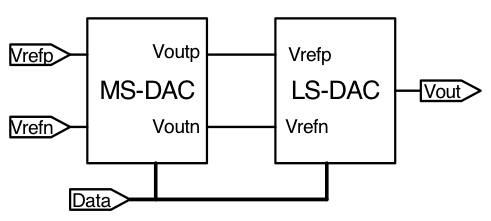
\includegraphics[width=6cm, height = 4cm]{pictures/kaskadiertDAC}
\end{minipage}
&

\begin{minipage}{8cm}
\begin{itemize}
  \item MS-DAC hat 2 Ausgangsspannungen (Über und unter dem gewünschten
  $V_{Out}$)
  \item LS-DAC hat kleine Eingangspannungsdifferenz $\to$ höhere Auflösung der
  Spannung
\end{itemize}
\end{minipage}
\\
\hline
\begin{minipage}{4cm}
\textbf{Zyklisch, algorithmischer DAC} \hartl{466}
\end{minipage}
&
\begin{minipage}{6cm}
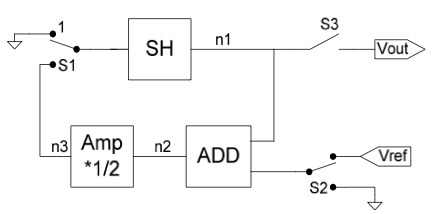
\includegraphics[width=6cm, height = 3cm]{pictures/zyklischDAC}
\end{minipage}
&

\begin{minipage}{8cm}
\textbf{Ablauf der Wandlung}\\
\begin{enumerate}
  \item Die Spannung im S/H wird gelöscht (Schalter S1), S3 geöffnet)
  \item Schalter S1 wird danach auf den Verstärker-Ausgang geschaltet
  \item Laufvariale k wird auf 0 gesetzt
  \item Schalter S2 wird gesetzt: VREF oder GND ( abh. $D_{K}$).
  \item Der Addierer generiert sein Ausgangssignal
  \item Der Verstärker generiert sein Ausgangssignal
  \item Im S/H wird die Feedback-Spannung gespeichert (S1)
  \item X wird um 1 erhöht
  \item Gehe zu Schritt 4, wenn $X\leq n$
\end{enumerate}
\end{minipage}
\\
\hline
\begin{minipage}{4cm}
\textbf{Pipelined DAC}\\
\end{minipage}
&
\begin{minipage}{6cm}
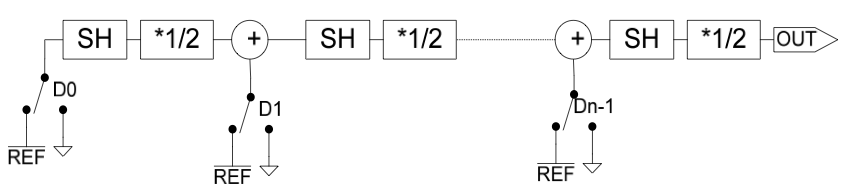
\includegraphics[width=6cm, height = 2cm]{pictures/piplinedDAC}
\end{minipage}
&

\begin{minipage}{8cm}
Die Latenz beträgt n Zyklen, die Update-Frequenz ist aber n-mal grösser
\end{minipage}
\\
\hline
\begin{minipage}{4cm}
\textbf{Strom-DAC}
\end{minipage}
&
\begin{minipage}{6cm}
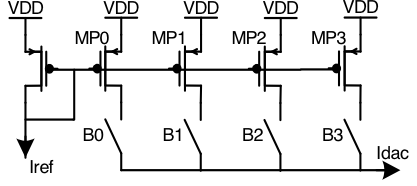
\includegraphics[width=6cm, height = 4cm]{pictures/stromDAC}
\end{minipage}
&

\begin{minipage}{8cm}
\begin{itemize}
  \item Stromspiegel
  \item MP0 ist gleich breit wie Stromquellen-MOS $\to$ I(MP0)=Iref
  \item MP1 ist doppelt so breit wie MP0 $\to I(MP1)=2*Iref$
  \item MP2 ist doppelt so breit wie MP1 $\to I(MP2)=4*Iref$
  \item \ldots
\end{itemize}
\end{minipage}
\\
\hline
\end{longtable}



\subsection{Multiplizierender DAC} \hartl{470}
\subsection{Auswahl von DACS} \hartl{470}
\begin{itemize}
  \item bei schnellen hochauflösenden Wandler werden Verfahren kombiniert
  \item für optimale Resultate müssen Kompromisse eingegangen werden
\end{itemize}
